\documentclass[a4paper]{article}
\usepackage[left=1.5cm, right=1.5cm, top=1.5cm, bottom=1.5cm, nohead, bindingoffset=0cm]{geometry}
\usepackage[T2A]{fontenc}
\usepackage[utf8]{inputenc}
\usepackage[english, russian]{babel}
\usepackage{setspace, amsmath}
\usepackage{cmap}
\usepackage{indentfirst}
\usepackage{color}   %May be necessary if you want to color links
\usepackage{hyperref}
\hypersetup{
    colorlinks=true, %set true if you want colored links
    linktoc=all,     %set to all if you want both sections and subsections linked
    linkcolor=black,  %choose some color if you want links to stand out
}
% collection-fontsrecommended and collection-fontsextra

\usepackage{listings}
\usepackage{xcolor}
\definecolor{commentgreen}{RGB}{2,112,10}
\definecolor{eminence}{RGB}{108,48,130}
\definecolor{weborange}{RGB}{255,165,0}
\definecolor{frenchplum}{RGB}{129,20,83}

\usepackage{graphicx}
\graphicspath{{pictures/}}
\DeclareGraphicsExtensions{.pdf,.png,.jpg}


\lstset { %
	language=Python,
	basicstyle=\small\sffamily, % размер и начертание шрифта для подсветки кода
	numbers=left,               % где поставить нумерацию строк (слева\справа)
	numberstyle=\tiny,           % размер шрифта для номеров строк
	stepnumber=1,                   % размер шага между двумя номерами строк
	numbersep=5pt,                % как далеко отстоят номера строк от подсвечиваемого кода
	backgroundcolor=\color{white}, % цвет фона подсветки - используем \usepackage{color}
	commentstyle=\color{commentgreen},
	keywordstyle=\color{eminence},
	showspaces=false,            % показывать или нет пробелы специальными отступами
	showstringspaces=false,      % показывать или нет пробелы в строках
	showtabs=false,             % показывать или нет табуляцию в строках
	frame=single,              % рисовать рамку вокруг кода
	tabsize=4,                 % размер табуляции по умолчанию равен 2 пробелам
	captionpos=t,              % позиция заголовка вверху [t] или внизу [b] 
	breaklines=true,           % автоматически переносить строки (да\нет)
	breakatwhitespace=false, % переносить строки только если есть пробел
	escapeinside={\%*}{*)}   % если нужно добавить комментарии в коде
}


\begin{document}
\fontsize{14pt}{18pt}\selectfont
	

\begin{center}
	\hfill \break
	\large{Санкт-Петербургский Государственный Университет}\\ 
	\hfill \break
	\large{Факультет Прикладной Математики и Процессов Управления}\\
	\hfill \break
	\hfill \break
	\hfill \break
	\hfill \break
	\begin{huge}{\textbf{
		Задание по эмпирическому анализу алгоритма по курсу \\
		\hfill \break
		«Алгоритмы и анализ сложности»\\
		\hfill \break
		Алгоритм LSD-поразрядной сортировки\\
	}}\end{huge}
	\hfill \break
	\hfill \break
	\hfill \break
	\hfill \break
	\hfill \break
	\hfill \break
\end{center}

\hfill \break
\hfill \break

\begin{center}
	\large{
		\begin{tabular}{lr}
			Преподаватель: & Никифоров К. А. \\\\
			Выполнил:      & студент группы 16.Б13-пу Кириченко В. В. \\
		\end{tabular}
	}\\
\end{center}

\vspace*{\fill}

\begin{center} Санкт-Петербург, 2018 \end{center}
\thispagestyle{empty}

\newpage

\tableofcontents

\newpage

\section{Описание и области применения алгоритма}
Алгоритм LSD-поразрядной сортировки является одним из вариантов алгоритма поразрядной сортировки. В нём числа сортируются по разрядам, причём сначала сортируются младшие разряды, а затем старшие. Данный алгоритм применялся для сортировки перфокарт. Алгоритм применялся в работе Германа Холлерита над табуляторами в 1887 году. Компьютерная реализация алгоритма была разработана в 1954 году Гарольдом Сьюардом.

\section{Математический анализ алгоритма}
В ходе работы алгоритму необходимо сортировать массив элементов для каждого разряда. Для этого числа распределяются по корзинам в соответствии с рассматриваемым разрядом, а затем корзины склеиваются. В таком случае основной операцией в ходе работы алгоритма является помещение элемента в корзину (список или массив). Таким образом, сложность алгоритма составляет $O(wn)$, где $n$ — число элементов в списке, а $w$ — количество разрядов.

\section{Характеристики входных данных и способ измерения трудоёмкости}
Входными данными для алгоритма является массив чисел. Трудоёмкость алгоритма измерялась в миллисекундах, затраченных на сортировку массива алгоритмом. Измерение времени производилось с помощью встроенного в стандартную библиотеку языка модуля time. Массивы генерировались с различным количеством как чисел, так и разрядов в каждом числе. Для упрощения интерпретации результатов измерения трудоёмкости в массиве присутствовали числа только с одинаковым количеством разрядов. Было выбрано следующее количество чисел в массиве: 100, 200, 400, 800, 1600, 3200, 6400, 12800, 25600, 51200; количество разрядов в каждом числе: 1, 2, 4, 8.

\section{Реализация алгоритма}
Алгоритм LSD-поразрядной сортировки был реализован на языке Python версии 3.7.1. Массив чисел представлен в виде списка. Для сортировки чисел по разрядам используются дополнительные списки. Их количество равно основанию системы счисления рассматриваемых чисел.
\\
\begin{lstlisting}
from math import log
 

def get_digit(num, base, digit_num):
    # pulls the selected digit
    return (num // base ** digit_num) % base  
 

def make_blanks(size):
    # create a list of empty lists to hold the split by digit
    return [[] for i in range(size)]  
 

def split(a_list, base, digit_num):
    buckets = make_blanks(base)
    for num in a_list:
        # append the number to the list selected by the digit
        buckets[get_digit(num, base, digit_num)].append(num)  
    return buckets

 
# concatenate the lists back in order for the next step
def merge(a_list):
    new_list = []
    for sublist in a_list:
       new_list.extend(sublist)
    return new_list

 
def max_abs(a_list):
    # largest abs value element of a list
    return max(abs(num) for num in a_list)

 
def split_by_sign(a_list):
    # splits values by sign - negative values go to the first bucket,
    # non-negative ones into the second
    buckets = [[], []]
    for num in a_list:
        if num < 0:
            buckets[0].append(num)
        else:
            buckets[1].append(num)
    return buckets

 
def radix_sort(a_list, base):
    # there are as many passes as there are digits in the longest number
    passes = int(round(log(max_abs(a_list), base)) + 1) 
    new_list = list(a_list)
    for digit_num in range(passes):
        new_list = merge(split(new_list, base, digit_num))
    return merge(split_by_sign(new_list))
	
\end{lstlisting}

\section{Генерация входных данных}
Генерация массивов чисел осуществляется на основе двух параметров — количества элементов в результирующем массиве и количества разрядов чисел (задаётся в виде минимального числа). Для генерации псевдослучайных равномерно распределённых чисел используется встроенный в стандартную библиотеку модуль random, реализованный на основе Вихря Мерсенна. Благодаря этому ГПСЧ лишён многих недостатков, присущих другим ГПСЧ, таких как малый период, предсказуемость и легко выявляемые статистические закономерности.
\begin{lstlisting}
def generate(length, amount):
    return [random.randint(length, 10 * length - 1) for _ in range(amount)]
\end{lstlisting}
\newpage
\section{Вычислительный эксперимент в исследуемом диапазоне входных данных}
С помощью описанного выше генератора данных было произведено тестирование алгоритма со всеми возможными парами параметров, указанных в разделе 3. На каждой такой паре алгоритм запускался 2000 раз с различными сгенерированными данными, чтобы минимизировать влияние как фоновых процессов, так и особенностей случайных данных. Результаты таких тестовых прогонов усреднялись и записывались в качестве результата.
\begin{lstlisting}
def timer(length, amount, number=2000):
    times = []
    for _ in range(number):
        to_sort = generate(length, amount)
        start = time.time()
        algorithm.radix_sort(to_sort, 10)
        stop = time.time()
        times.append(stop - start)
    return sum(times) / number
    

lengths = [1, 10, 1000, 10000000]
amounts = [100, 200, 400, 800, 1600, 3200, 6400, 12800, 25600, 51200]

def test():
    tested = list()
    for length in lengths:
        for amount in amounts:
            ex_time = timer(length, amount)
            tested.append({'from': length,
                           'to': 10 * length,
                           'amount': amount,
                           'time': ex_time * 1000})
    return tested
\end{lstlisting}

\section{Анализ полученных результатов}
В \hyperref[table1]{таблицах 1–4} представлены результаты, полученные в ходе вычислительного эксперимента.
\begin{center}
	\label{table1}
\begin{tabular}{|c|c|}
	\hline
	Количество элементов & Время работы, мс \\
	\hline
	100 & 0.0668172836303711 \\ \hline
	200 & 0.14360392093658447 \\ \hline
	400 & 0.28176605701446533 \\ \hline
	800 & 0.555321455001831 \\ \hline
	1600 & 1.2162401676177979 \\ \hline
	3200 & 2.363770008087158 \\ \hline
	6400 & 4.941829562187195 \\ \hline
	12800 & 9.466262340545654 \\ \hline
	25600 & 18.687508702278137 \\ \hline
	51200 & 37.44811272621155 \\ \hline
\end{tabular} \\
\hfill \break
	Таблица 1. Массивы чисел с 1 разрядом.
	\label{table2}
\begin{tabular}{|c|c|}
	\hline
	Количество элементов & Время работы, мс \\
	\hline
	100 & 0.09697568416595459 \\ \hline
    200 & 0.22541213035583496 \\ \hline
    400 & 0.4338417053222656 \\ \hline
    800 & 0.9395959377288818 \\ \hline
    1600 & 1.827741265296936 \\ \hline
    3200 & 3.6263442039489746 \\ \hline
    6400 & 6.917779326438904 \\ \hline
    12800 & 14.10499358177185 \\ \hline
    25600 & 28.16263520717621 \\ \hline
    51200 & 56.175602436065674 \\ \hline
\end{tabular} \\
\hfill \break
	Таблица 2. Массивы чисел с 2 разрядами.
	\break \hfill \break
	\label{table3}
\begin{tabular}{|c|c|}
	\hline
	Количество элементов & Время работы, мс \\
	\hline
	100 & 0.19944369792938232 \\ \hline
    200 & 0.3894462585449219 \\ \hline
    400 & 0.7644665241241455 \\ \hline
    800 & 1.5598496198654175 \\ \hline
    1600 & 3.0463205575942993 \\ \hline
    3200 & 6.123116374015808 \\ \hline
    6400 & 12.208956241607666 \\ \hline
    12800 & 24.4019957780838 \\ \hline
    25600 & 48.945778012275696 \\ \hline
    51200 & 98.92793309688568 \\ \hline
\end{tabular} \\
\hfill \break
	Таблица 3. Массивы чисел с 4 разрядами.
	\break \hfill \break
	\label{table4}
\begin{tabular}{|c|c|}
	\hline
	Количество элементов & Время работы, мс \\
	\hline
	100 & 0.3834867477416992 \\ \hline
    200 & 0.7435144186019897 \\ \hline
    400 & 1.435721755027771 \\ \hline
    800 & 2.9485440254211426 \\ \hline
    1600 & 5.750182867050171 \\ \hline
    3200 & 11.492654204368591 \\ \hline
    6400 & 23.274991035461426 \\ \hline
    12800 & 46.117165088653564 \\ \hline
    25600 & 92.64567613601685 \\ \hline
    51200 & 187.23099100589752 \\ \hline
\end{tabular} \\
\hfill \break
	Таблица 4. Массивы чисел с 8 разрядами.
\end{center}
\newpage
Найдём аппроксимацию функции трудоёмкости алгоритма $aw^bn^c+d$ при помощи функции FindFit из пакета Wolfram Mathematica: $a=0.000519248, b=0.851639, c=1.01574, d=0.30329$. На рисунках \hyperref[image1]{1} и \hyperref[image2]{2} можно видеть, что найденная аппроксимация близка к полученным данным. Можно сделать вывод, что количество разрядов в числах влияют не столь существенно по сравнению с количеством элементов в массиве. Тем не менее, полученная оценка трудоёмкости близка к оценке, полученной в ходе математического анализа алгоритма.
\begin{figure}[!]
	\center{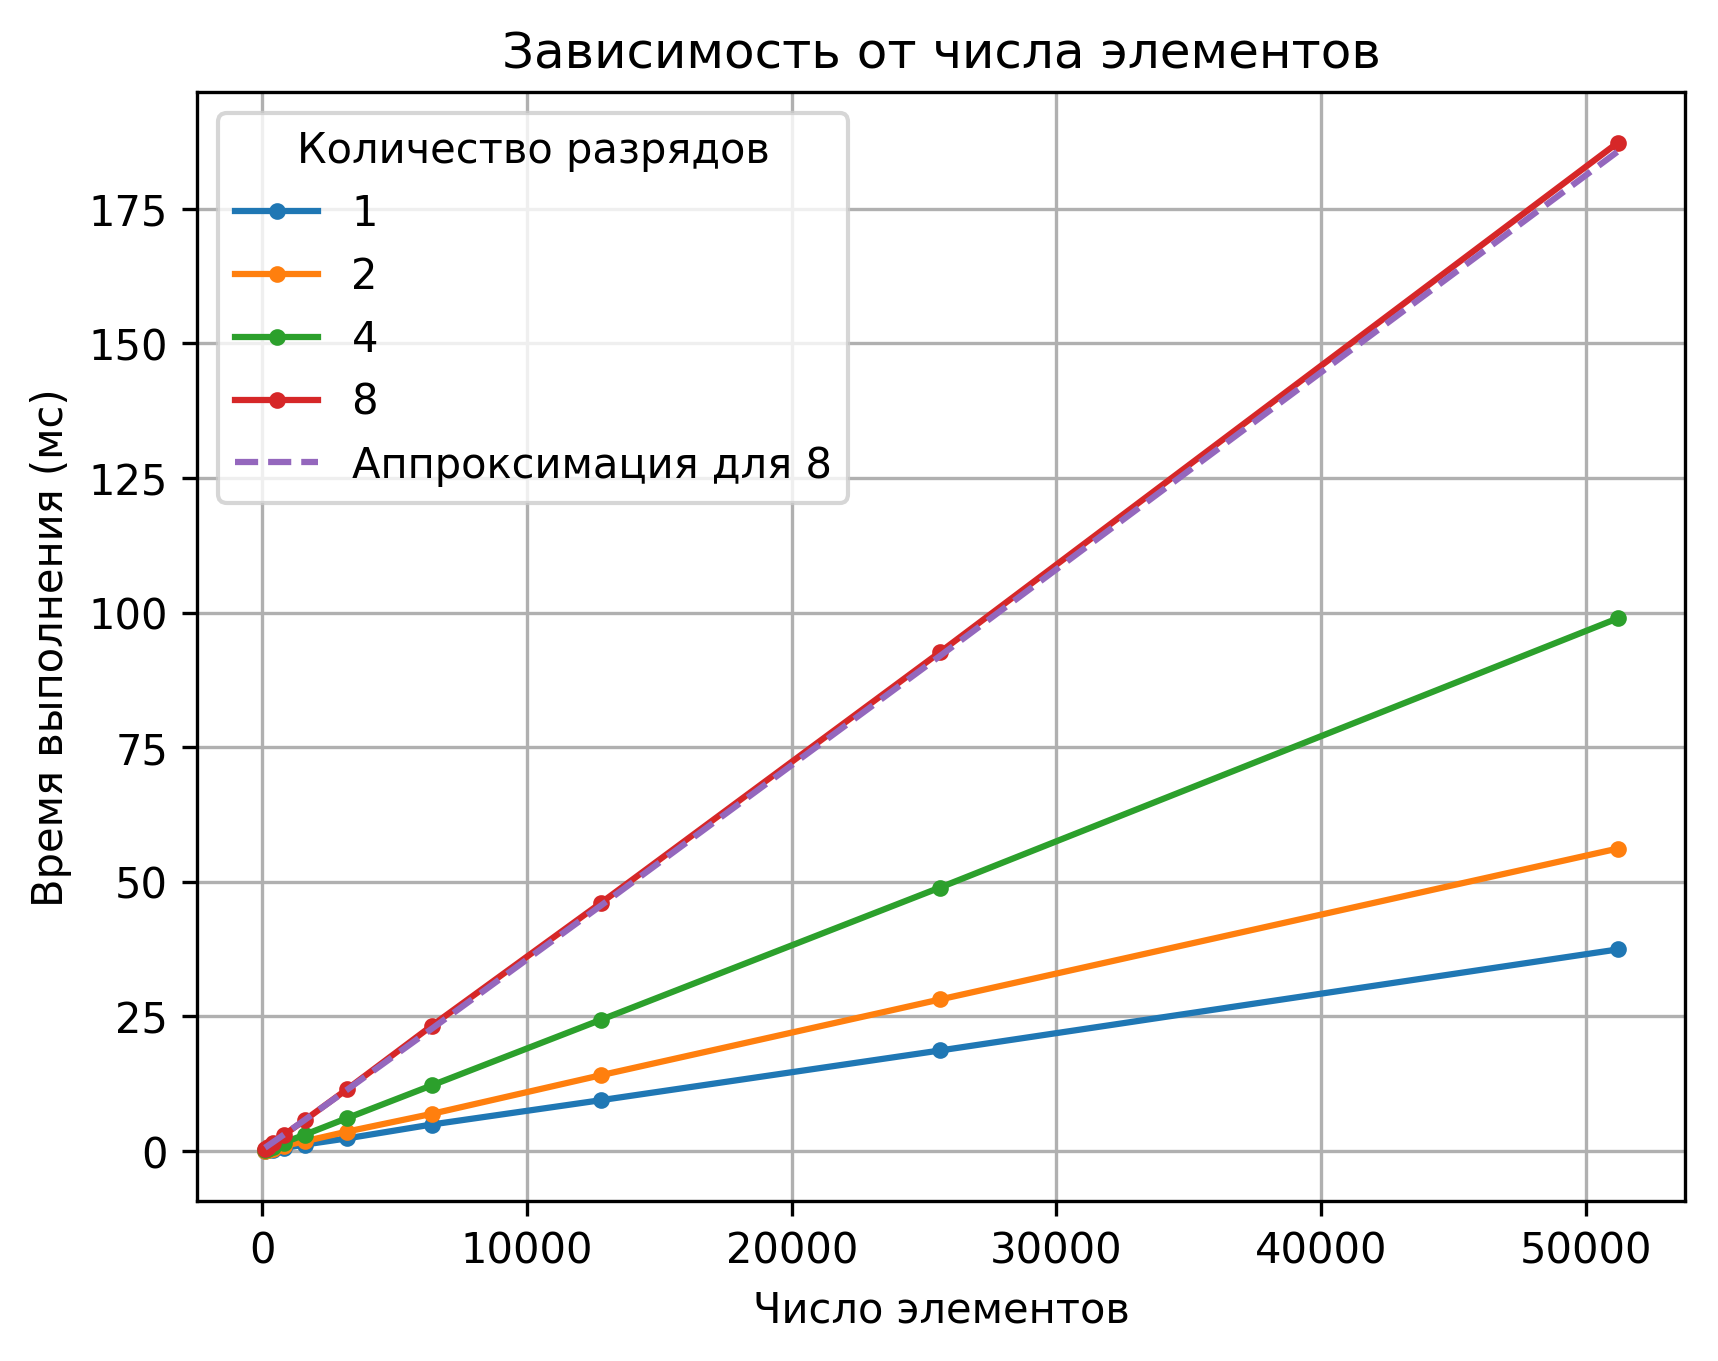
\includegraphics{amount.png}}
	\caption{зависимость времени выполнения от числа элементов}
	\label{image1}
\end{figure}

\begin{figure}[!]

\center{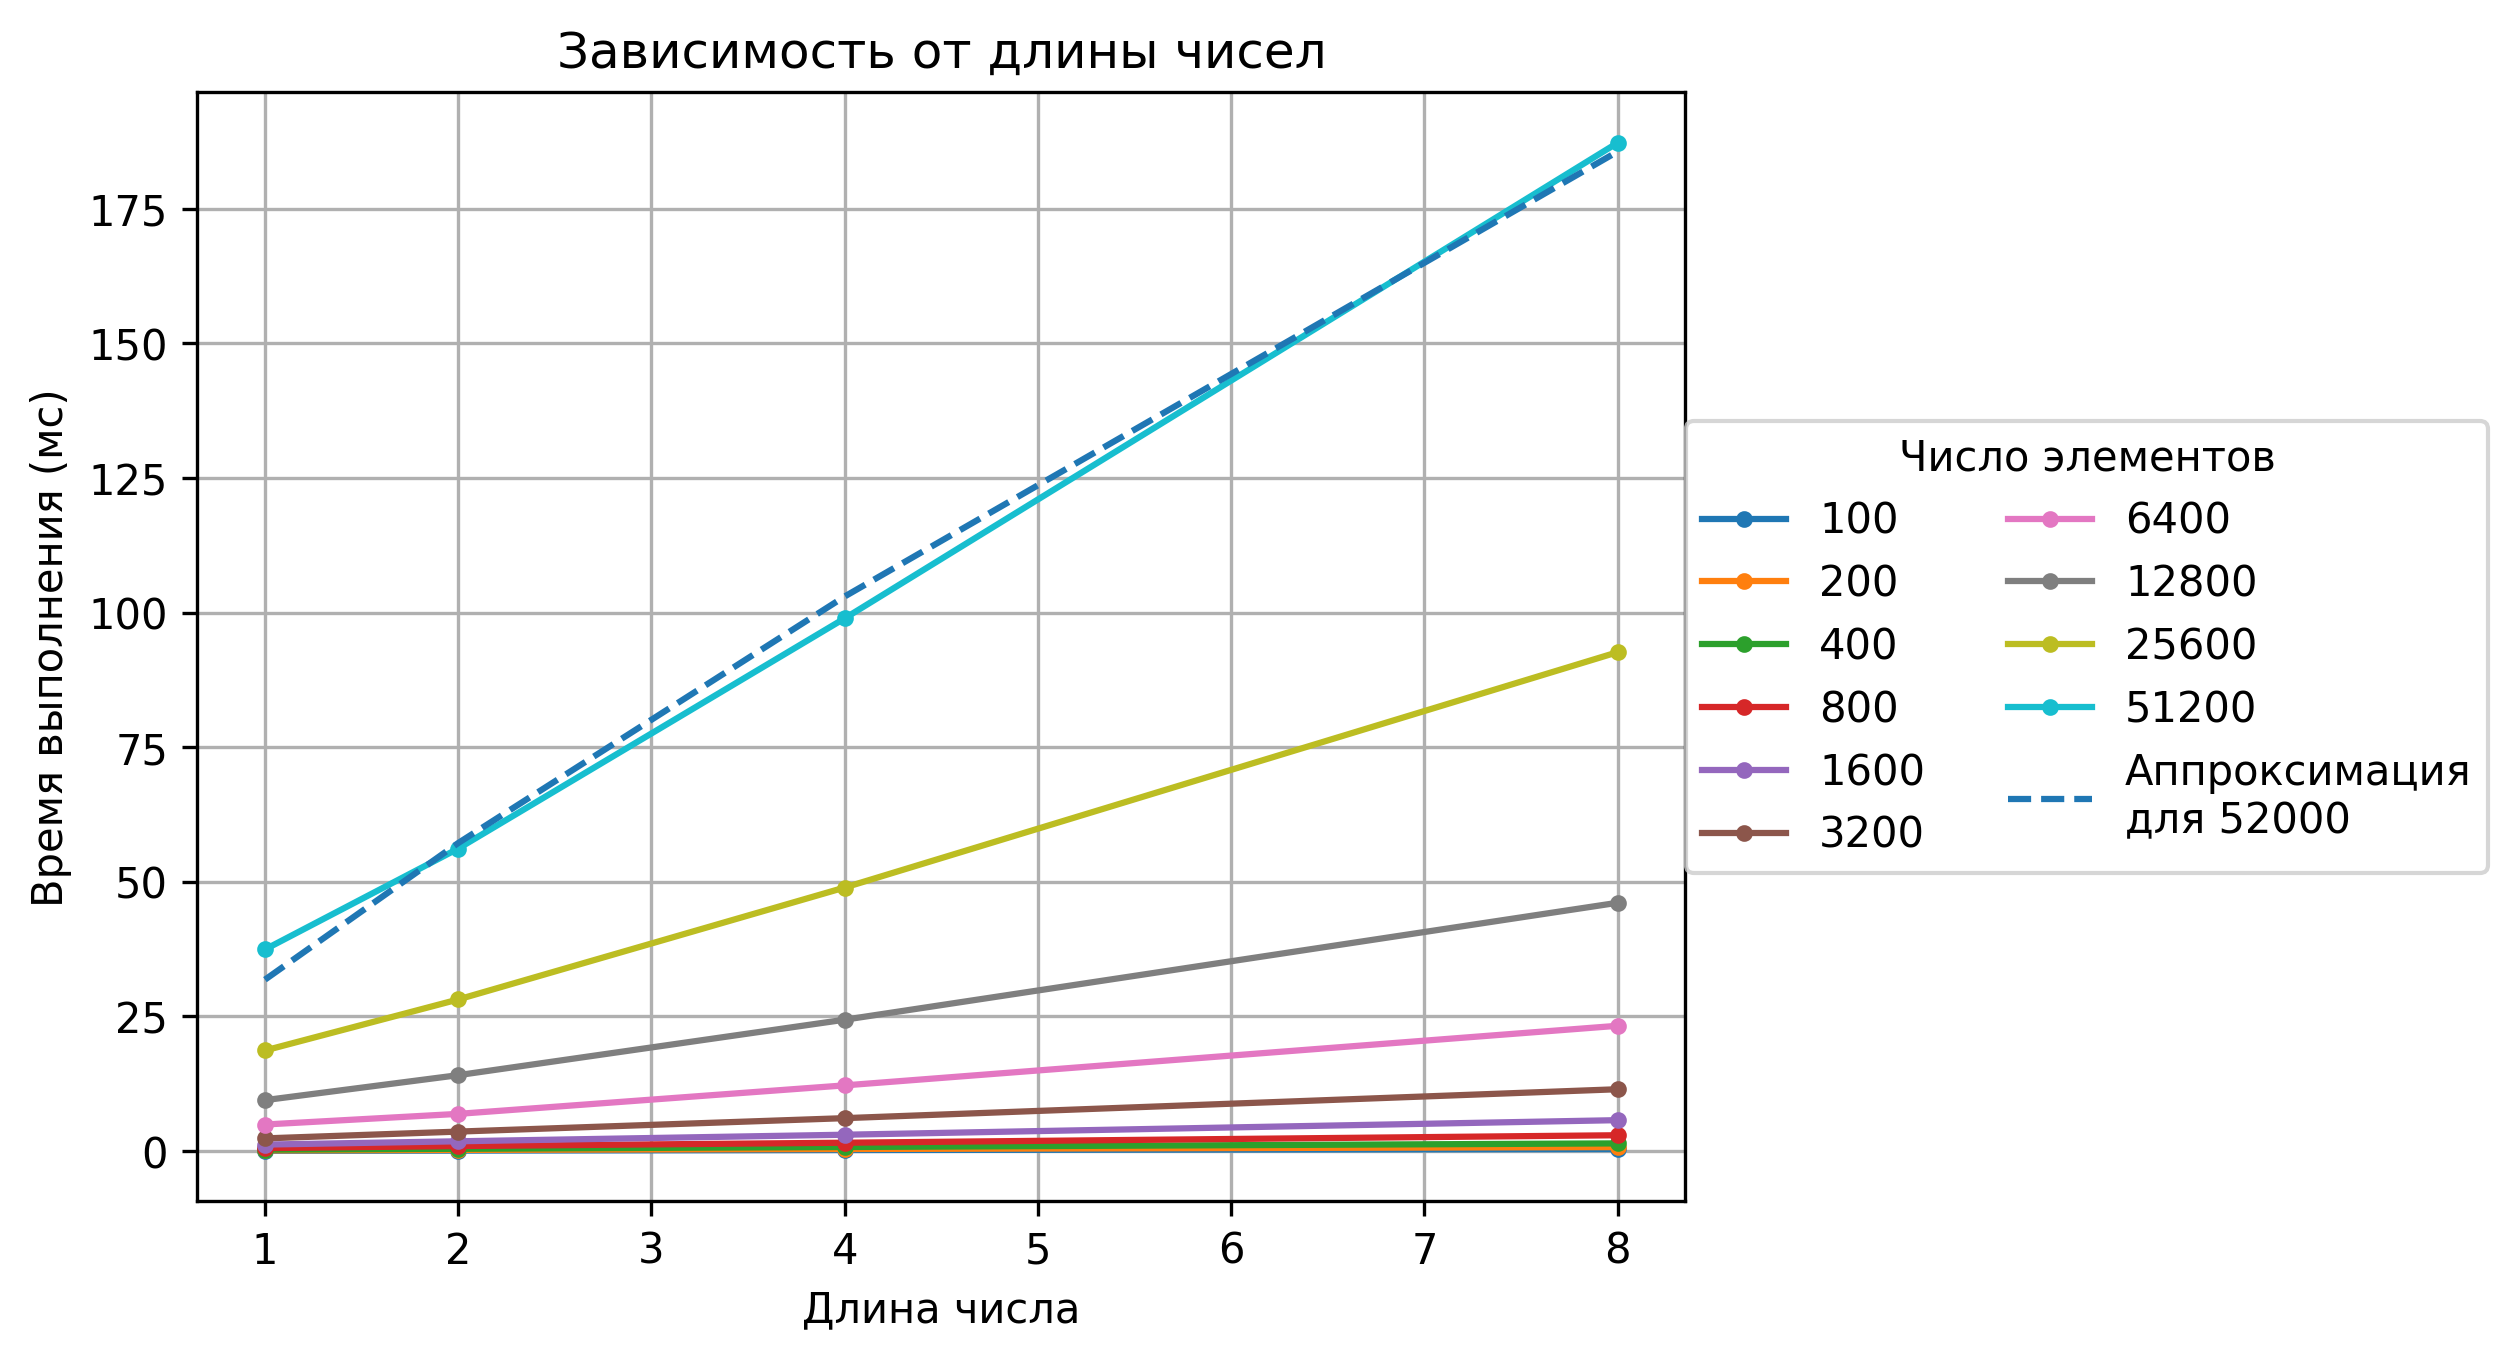
\includegraphics[width=\textwidth,height=\textheight,keepaspectratio]{length.png}}
	\caption{зависимость времени выполнения от количества разрядов}
	\label{image2}
\end{figure}

Проанализируем соотношение ${T(2n)\over{T(n)}}$ для массива чисел с 8 разрядами:
\begin{center}
\begin{tabular}{|c|c|}
	\hline
	Количество элементов $n$ & ${T(2n)\over{T(n)}}$ \\
	\hline
	100 & 1.93882689 \\ \hline
    200 & 1.93099383 \\ \hline
    400 & 2.053701572 \\ \hline
    800 & 1.950177042 \\ \hline
    1600 & 1.998658907 \\ \hline
    3200 & 2.025205894 \\ \hline
    6400 & 1.981404204 \\ \hline
    12800 & 2.008919585 \\ \hline
    25600 & 2.020936096 \\ \hline
\end{tabular}
\end{center}
Во всех случаях соотношение ${T(2n)\over{T(n)}}$ соответствует примерно 2. Это означает, что увеличение количества чисел в массиве линейно влияет на трудоёмкость алгоритма. Аналогично проанализируем влияние количества разрядов на примере массивов с 25600 элементов:
\begin{center}
\begin{tabular}{|c|c|}
	\hline
	Количество разрядов $w$ & ${T(2w)\over{T(w)}}$ \\
	\hline
	1 & 1.507029945 \\ \hline
    2 & 1.737968683 \\ \hline
    4 & 1.892822627 \\ \hline
\end{tabular}
\end{center}
Соотношение ${T(2w)\over{T(w)}}$ стремится к 2, поэтому можно сделать вывод, что количество разрядов чисел так же оказывает линейное влияние на трудоёмкость алгоритма.

\section{Список источников}

\begin{enumerate}
	\item \href{https://en.wikipedia.org/wiki/Radix_sort}[Radix Sort — Википедия];
	\item \href{http://algolist.manual.ru/sort/radix_sort.php}[Поразрядная сортировка — Manual.ru];
	\item Д. Э. Кнут. Искусство программирования, том 3. Сортировка и поиск — 2-е изд. — М.: И.Д.Вильямс, 2007. — C. 192–196;
	\item \href{https://docs.python.org/3/library/random.html}[Модуль random в Python 3]
	\item \href{https://docs.python.org/3/library/time.html}[Модуль time в Python 3]
	\item \href{http://www.rosettacode.org/wiki/Sorting_algorithms/Radix_sort#Python}[Реализация алгоритма на языке Python]
	\item \href{https://reference.wolfram.com/language/ref/FindFit.html}[Функция FindFit в Wolfram Mathematica]
\end{enumerate}

\section{Характеристики использованной вычислительной среды и оборудования}
В качестве вычислительной среды использовался интерпретатор CPython 3.7.1, запущенный на персональном компьютере со следующими характеристиками:
\begin{itemize}
	\item Процессор: Intel Core i7-8700K (6 ядер, 12 потоков, работал на тактовой частоте 4.35 ГГц, L1-кэш: 384 КиБ, L2-кэш: 1.5 МиБ, L3-кэш: 12 МиБ)
	\item Оперативная память: 16 ГиБ DDR3 3200 МГц в двухканальном режиме
	\item Графический ускоритель: NVIDIA GeForce GTX 1070 (8 ГиБ видеопамяти GDDR5)
	\item Операционная система: Microsoft Windows 10.
\end{itemize}

\end{document}